%    Latex Template for ACA 2015
%%%%%%%%%%%%%%%%%%%%%%%%%%%%%%%%%%%%%%%%
%    DO NOT CHANGE THE SETTINGS BELOW
%%%%%%%%%%%%%%%%%%%%%%%%%%%%%%%%%%%%%%%%
\documentclass[11pt]{article}
\usepackage{epsfig}
\usepackage{graphicx}
\usepackage[latin1]{inputenc}
\usepackage[T1]{fontenc}
\usepackage{mathptmx}
\usepackage{url}



\begin{document}



%%%%%%%%%%%%%%%%%%%%%%%%
%%%%%%%%%%%%%%%%%%%%%%%%%%%%%%%%%%%%%%%%
%    DO NOT CHANGE THE SETTINGS ABOVE
%%%%%%%%%%%%%%%%%%%%%%%%%%%%%%%%%%%%%%%%
%
\vspace{-0.8cm}
\begin{flushleft}
\Large \textbf{\noindent
%%% PLEASE INSERT THE TITLE OF YOUR TALK HERE %%%%%%%
A Transparent Rule Based CAS to support Formalization of Knowledge}
%%%%%%%%%%%%%%%%%%%%%%%%%%%%%%%%%%%%%%%%%%%%%%%%%%%%%%%%
\\
%%%%%%%%%%%%%%%%%%%%%%%%%%%%%%
\vspace{0.5cm}
\normalsize
 %%%%%%             NAMES OF AUTHORS         %%%%%%
 %%%%%% NAME OF SPEAKER SHOULD BE UNDERLINED %%%%%%%%%
\normalsize{
 %%%%%% FOR EXAMPLE %%%%%
 \underline{R. Oldenburg}$^1$
 %%%%%%%%%%%%%%%%%%%%%%%%
} \\
\vspace{5mm}
\textit{\footnotesize
 %%%%%% AFFILIATION OF AUTHORS %%%%%%
$^1$ University of Augsburg, Germany,
reinhard.oldenburg@math.uni-augsburg.de\\
 %%%%%%%%%%%%%%%%%%%%%%%%%%%%%%%%%%%%%
}
\end{flushleft}


Algebra is an important and highly complicated subject of schools mathematics that can be structured according to various dimensions of analysis, e.g. it comprises different kinds of activities \cite{Ki} and structures that obey different linguistic systems \cite{HKO}. This paper is written in the spirit of that last reference and takes the linguistic view of mathematics to include syntactical, semantical and pragmatic aspects of the algebraic language. Syntactical aspects of algebra can easily be handled by computer algebra systems (CAS). However, there is evidence (e.g. \cite{OW} but many others) that students have great difficulty to understand what a CAS does and how its output is to be interpreted. Thus, we conducted a small developmental research project that aimed at producing a prototype of a CAS that is as transparent to students as possible. We hope that students can understand how this system works completely and furthermore, it is hoped that they can use it to formalise their mathematical knowledge by making the system more powerful by giving additional rules. So the ideas is to extend Papert's idea of the computer as a trainee to the realm of computer algebra. 
 
The system developed is called SCAS (simple syntactical CAS, doubling the S in the acronym was avoided for obvious reasons) aims to support the learning of syntactical aspects of algebra as well to provide a simple mental model of what a computer algebra system (CAS) is and how it works. 
The basic use of SCAS is similar to other CAS: You enter an expression and the system answers with an output. E.g. if you enter \texttt{2*x+y+x+3} then the system answers 	\texttt{3*x+y+3}. 

SCAS is a rule based term rewriting system \cite{BN}. Of course, modern CAS are not (completely) rule based as many operations have much more efficient algorithmic solutions than those possible by term rewriting. Nevertheless, we believe that this gives a good mental model of the syntactic way a CAS treats mathematical expressions.
  
The following simple rules govern the behaviour of the system:

\begin{itemize}
\item All expressions are represented by binary trees (e.g. \texttt{a+b+c} is interpreted as \texttt{a+(b+c)})
\item There is a list of rewrite rules. A rule consists of a pattern, possibly a condition, and a replacement. A handy notation is 
\textit{pattern}$\rightarrow$\textit{replacement}. The system goes through this list of rules and with each rule it checks if it can be applied to any sub-expression of the current expression. If so it checks if the condition of the rule is satisfied, and if this is the case the expression is replaced.
\item This process is repeated until no applicable rule is in the rule list. The final expression is send to the output.
\end{itemize}

Students can turn on or of indivudal rules like \texttt{A-A$\rightarrow$ 0} or rule groups (like that for expanding). Moreover, they can enter new rules. The idea is to give them the opportunity to formalize their knowlede e.g. about derivatives. The following screen shot shows the user interface. 

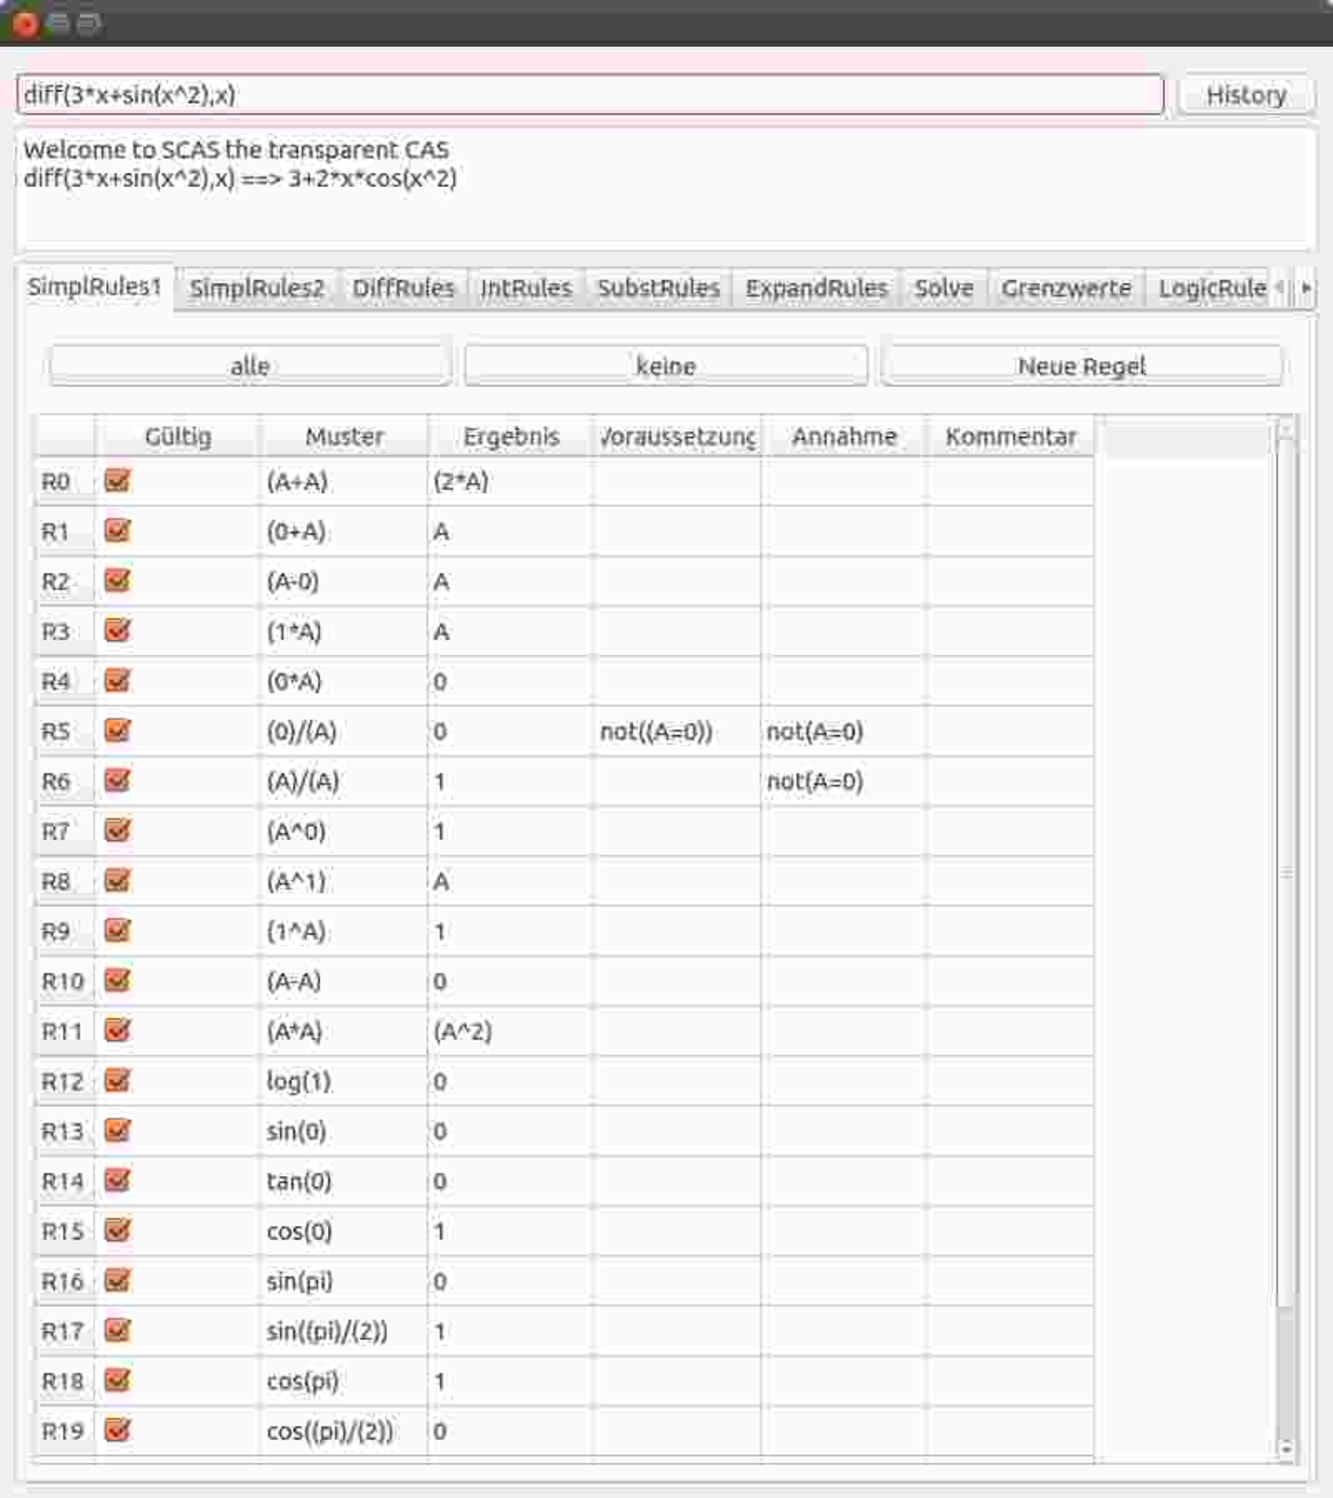
\includegraphics[scale=0.5]{OldenburgFig.pdf}

The talk will discuss the design ideas and show the system as well as further didactical questions.


%%%%%%%%%%%%%%%%%%%%%%%%%%%%%%%%%%%%%%%


%%%%%%%%%%%%%%%%%%%%%%%%%%%%%%%%%%%%%%%%
%% BIBLIOGRAPHY
%%%%%%%%%%%%%%%%%%%%%%%%%%%%%%%%%%%%%%%%
\begin{thebibliography}{00}
\addcontentsline{toc}{chapter}{References}
\setlength{\itemsep}{-1mm}
\footnotesize
\bibitem{BN} F. Baader, T. Nipkow, \textit{Term Rewriting and All That}, Cambridge UP, Cambridge (1999).
\bibitem{Ki} C. Kieran, \textit{The core of algebra: reflections on its main activities.},  in  K. Stacey et al. (eds.), The future of the teaching and learning of algebra. Kluwer Academic Publishers, Dordrecht (ISBN 1-4020-8130-8), pp. 21-33 (2004).
\bibitem{HKO} J. Hodgen, D. Kuechemann, R. Oldenburg, \textit{Syntactic and Semantic Items in Algebra Tests - A conceptual and empirical view},  CERME 2013. 
\bibitem{OW} R. Oldenburg, B. Weygandt, \textit{Einsatzm\"oglichkeiten und Grenzen von Computeralgebrasystemen zur F\"orderung der Konzeptentwicklung}, in A. Hoppenbrock et al. (eds.) Lehren und Lernen von Mathematik in der Studieneingangsphase. Springer, Berlin (2015).

\end{thebibliography}
\normalsize
\end{document} 
